\chapter{Simulación}

Se simularon las características del circuito en LTSpiceXVII.

\section{Circuito de Polarización}

\subsection{Carga Pasiva}
\begin{figure}[ht]
    \begin{minipage}[t]{0.43\textwidth}
        \centering
        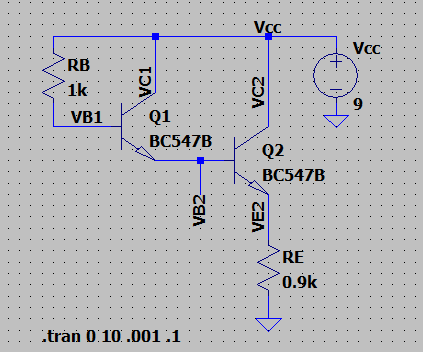
\includegraphics[width=\linewidth]{3_simulacion/fig/cir_pol_p.png}
        \caption{Circuito de Polarización configurado en LTSpiceXVII}
    \end{minipage}\hfill
    \begin{minipage}[t]{0.43\textwidth}
        \centering
        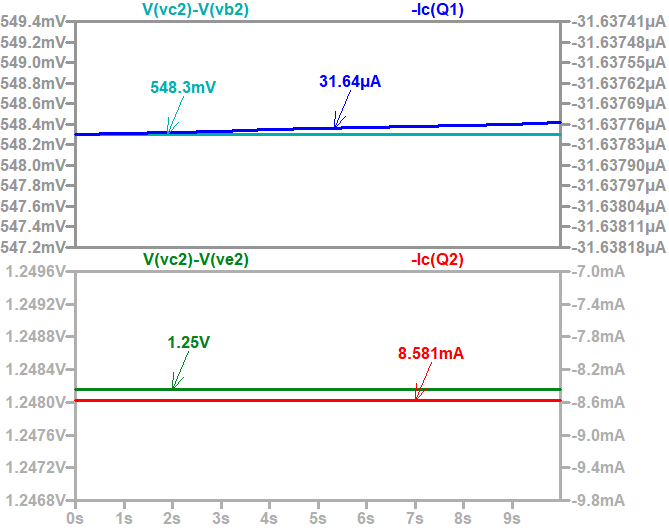
\includegraphics[width=\linewidth]{3_simulacion/fig/pol_pasiva.png}
        \caption{Punto de operación del circuito en CC}
    \end{minipage}
\end{figure}

\subsection{Carga Activa}
\begin{figure}[ht]
    \begin{minipage}[t]{0.43\textwidth}
        \centering
        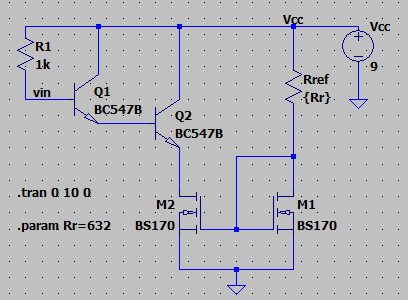
\includegraphics[width=\linewidth]{3_simulacion/fig/cir_pol_a.png}
        \caption{Circuito de Polarización configurado en LTSpiceXVII}
    \end{minipage}\hfill
    \begin{minipage}[t]{0.43\textwidth}
        \centering
        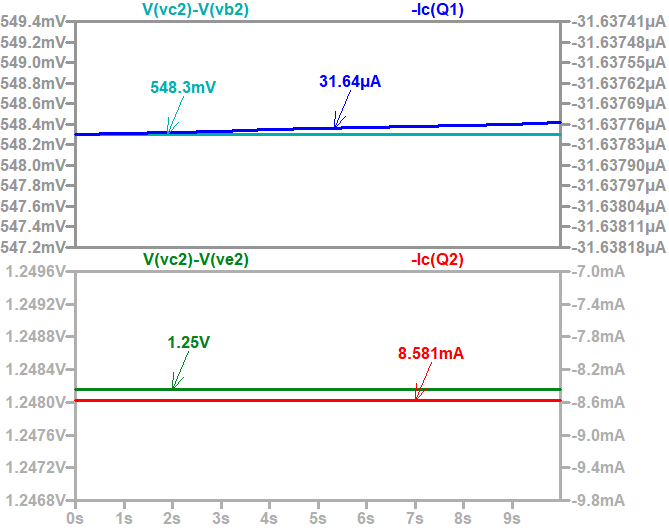
\includegraphics[width=\linewidth]{3_simulacion/fig/pol_pasiva.png}
        \caption{Punto de operación del circuito en CC}
    \end{minipage}
\end{figure}

\newpage
\section{Circuito Incremental}
Se simuló el comportamiento del circuito incremental primero con todos los componentes y como comparación con solo el modelo de pequeña señal.

\begin{figure}[ht]
    \begin{minipage}[t]{0.45\textwidth}
        \centering
        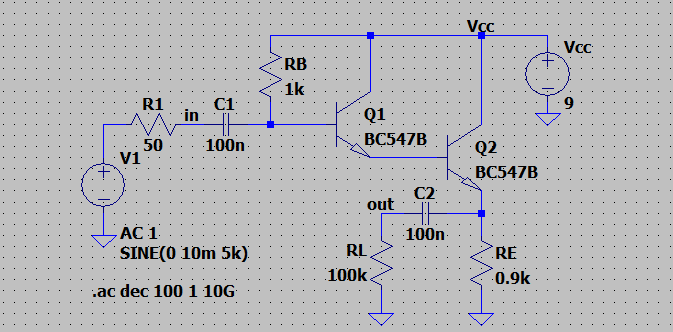
\includegraphics[width=\linewidth]{3_simulacion/fig/cir_comp_p.png}
        \caption{Circuito completo con carga pasiva}
    \end{minipage}\hfill
    \begin{minipage}[t]{0.45\textwidth}
        \centering
        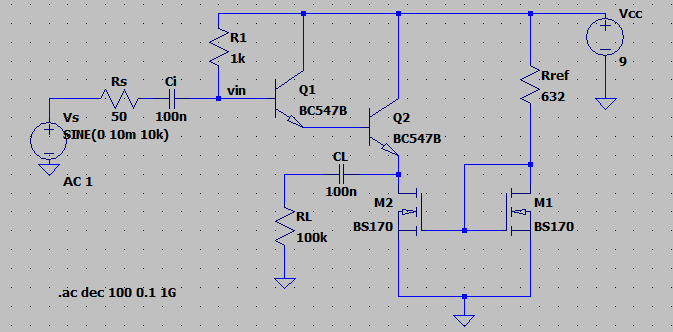
\includegraphics[width=\linewidth]{3_simulacion/fig/cir_comp_a.png}
        \caption{Circuito completo con carga activa}
    \end{minipage}
\end{figure}

\begin{figure}[ht]
    \centering
    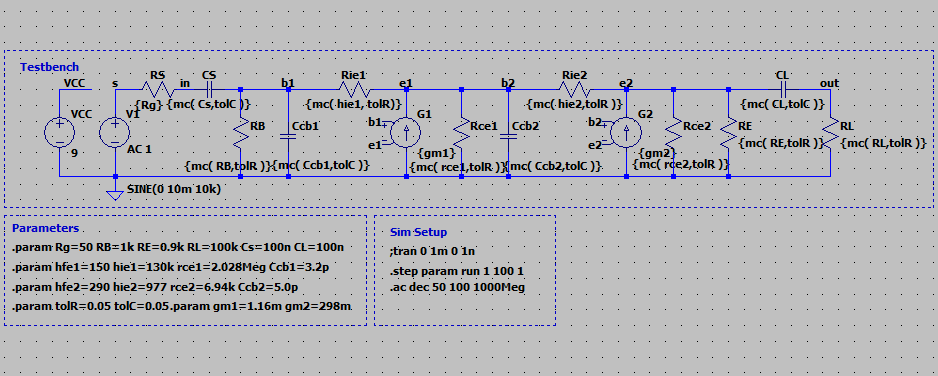
\includegraphics[width=\linewidth]{3_simulacion/fig/tb_1.png}
    \caption{Banco de prueba con modelo de pequeña señal}
\end{figure}

\begin{figure}[ht]
    \begin{minipage}[t]{0.48\textwidth}
        \centering
        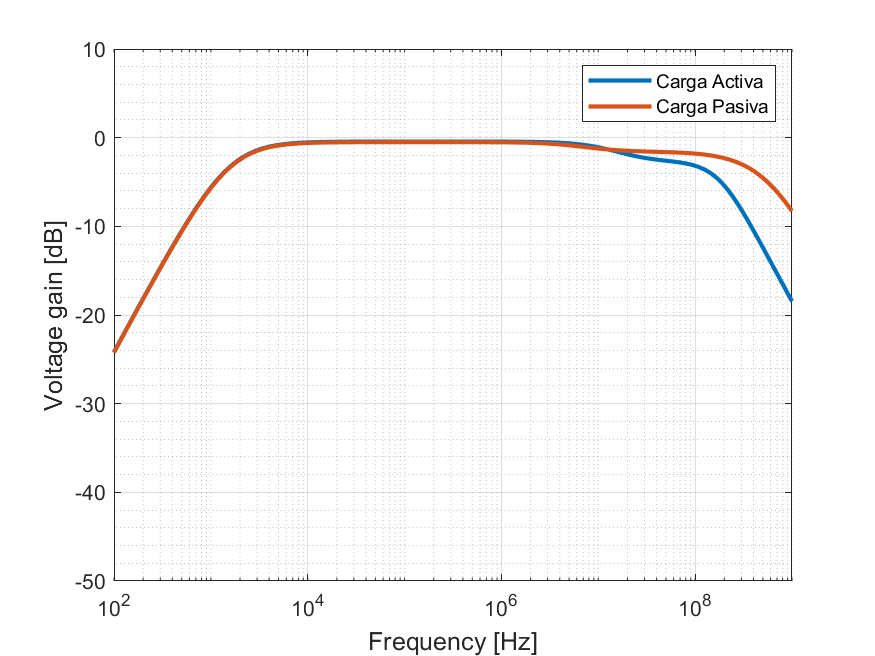
\includegraphics[width=\linewidth]{3_simulacion/fig/Bode_circuito.png}
        \caption{Respuesta en frecuencia de la ganancia de tensión de los circuitos}
        \label{fig:bode_cir}
    \end{minipage}\hfill
    \begin{minipage}[t]{0.48\textwidth}
        \centering
        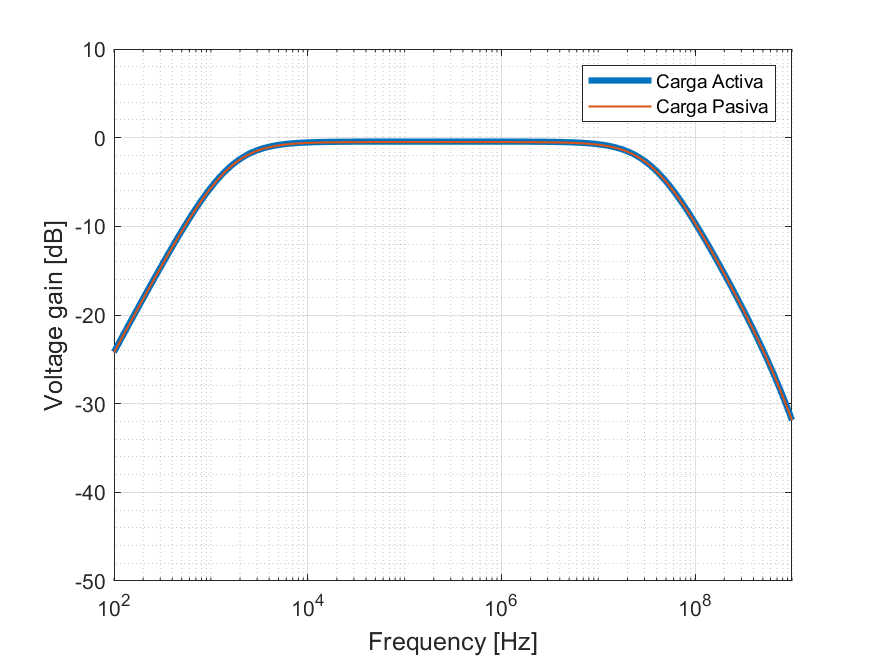
\includegraphics[width=\linewidth]{3_simulacion/fig/Bode_tb1.png}
        \caption{Respuesta en frecuencia de la ganancia de tensión del banco de prueba}
        \label{fig:bode_tb1}
    \end{minipage}
\end{figure}

Se puede observar una mejora en el circuito con carga activa al acortar el ancho de banda a altas frecuencias en la figura \ref{fig:bode_cir}. Por otro lado, hay una diferencia considerable entre la respuesta en frecuencia del circuito real y la del modelo incremental. Se encontró que esto ocurre por despreciar las capacitancias parásitas entre la base y el emisor.

Utilizando una nueva configuración donde se consideraron estas capacitancias, se obtuvo una simulación más acorde a la del circuito real (figura \ref{fig:bode_tb2}). Aún así, el circuito conserva su comportamiento de seguidor por emisor en las frecuencias medias.

Por último también se ejecutó el análisis de montecarlo para cada variación de los circuitos simulados. Se puede observar en cada caso cómo la aplicación de la carga activa en primer lugar acerca el polo dominante de alta frecuencia, reduciendo el ancho de banda.

\begin{figure}
    \centering
    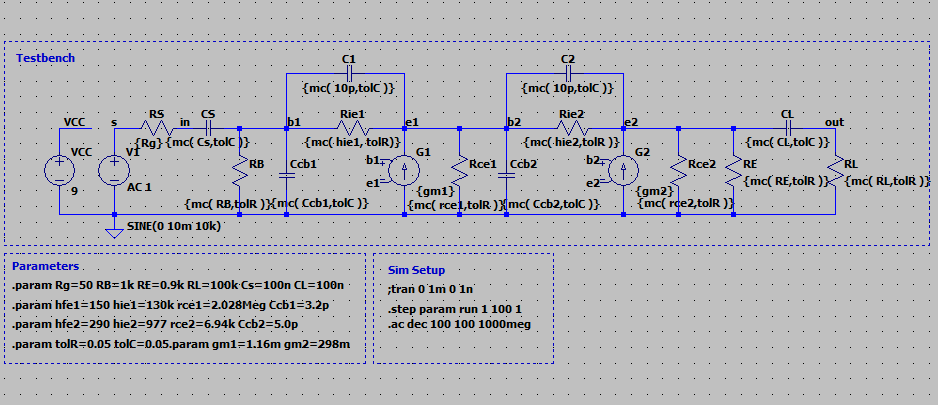
\includegraphics[width=\linewidth]{3_simulacion/fig/tb_2.png}
    \caption{Banco de pruebas con Capacitancias Base Emisor}
\end{figure}

\begin{figure}
    \centering
    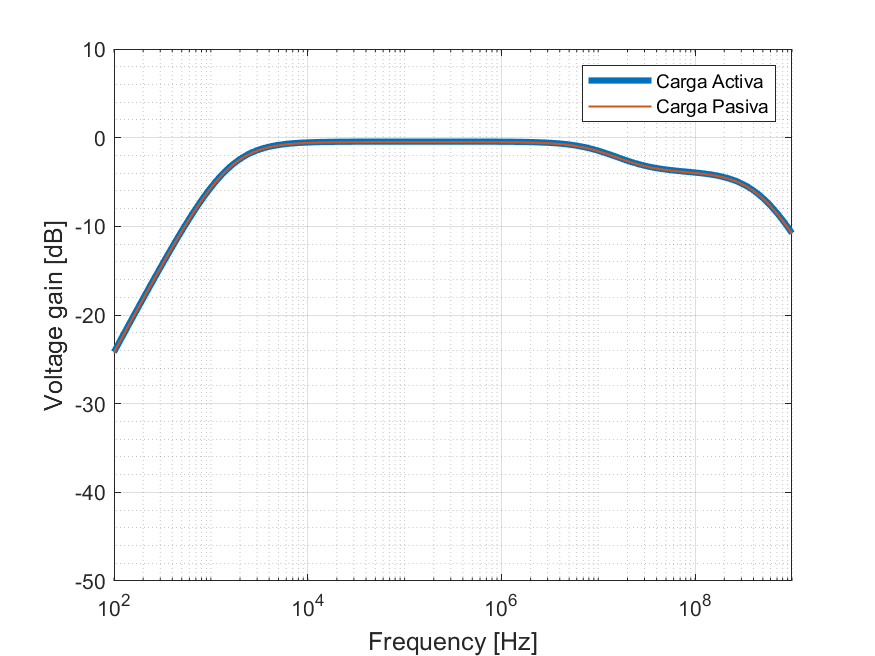
\includegraphics[width=0.5\linewidth]{3_simulacion/fig/Bode_tb2.png}
    \caption{Respuesta en frecuencia del banco de prueba con $C_{eb}$}
    \label{fig:bode_tb2}
\end{figure}

\begin{figure}
    \centering
    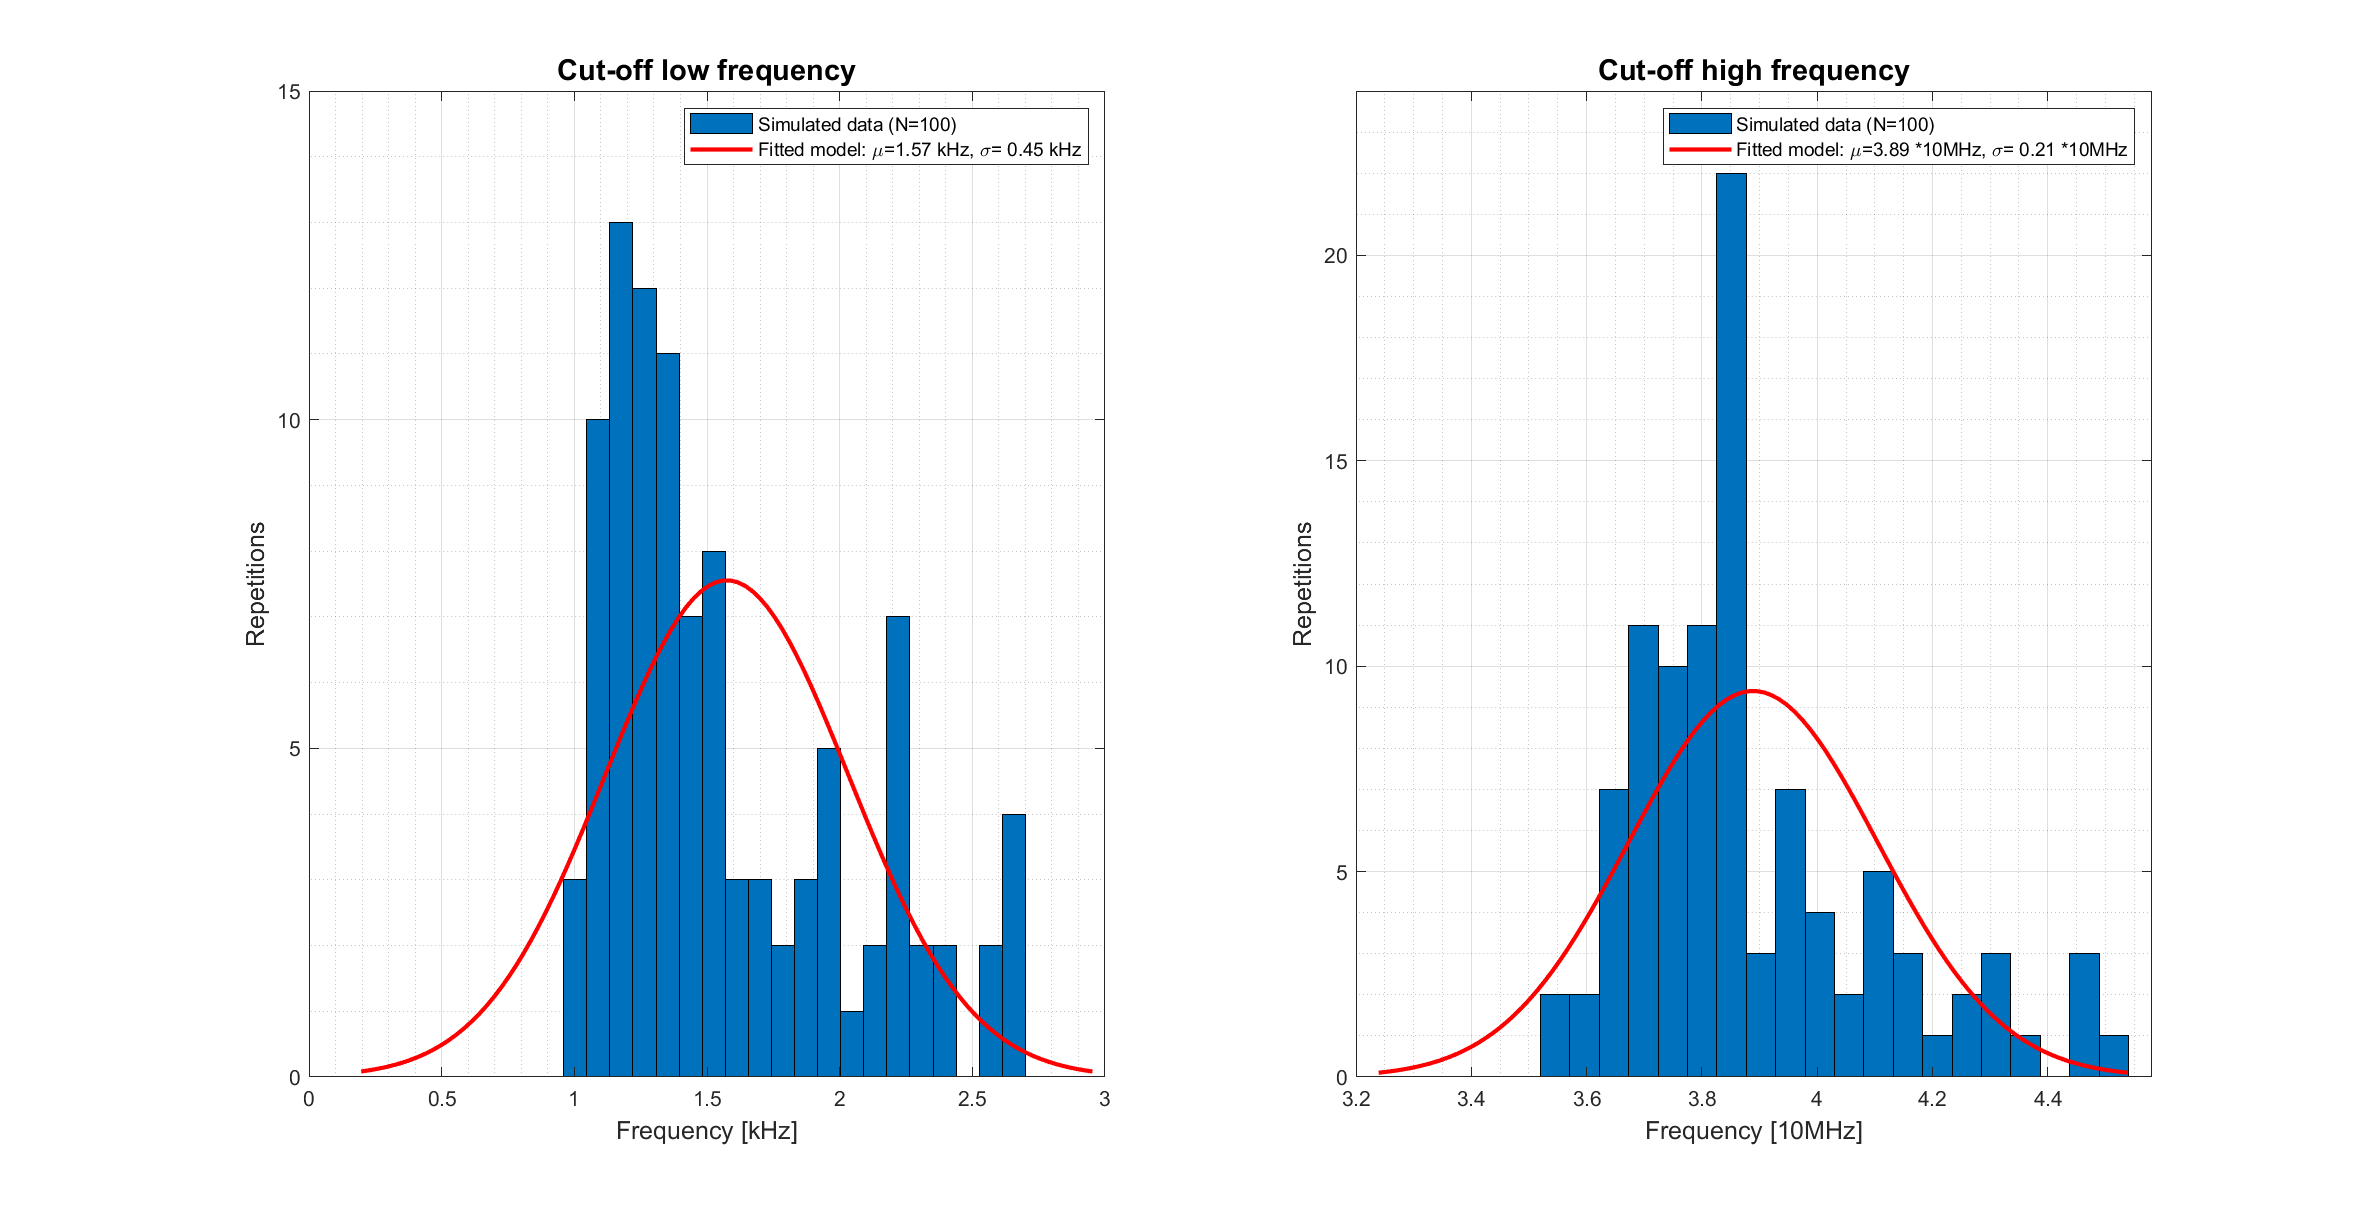
\includegraphics[width=\linewidth]{3_simulacion/fig/Hist_cir_pas_100.png}
    \caption{Análisis estadístico de los lugares de los polos de bajas y altas frecuencias con carga pasiva, circuito real}
\end{figure}

\begin{figure}
    \centering
    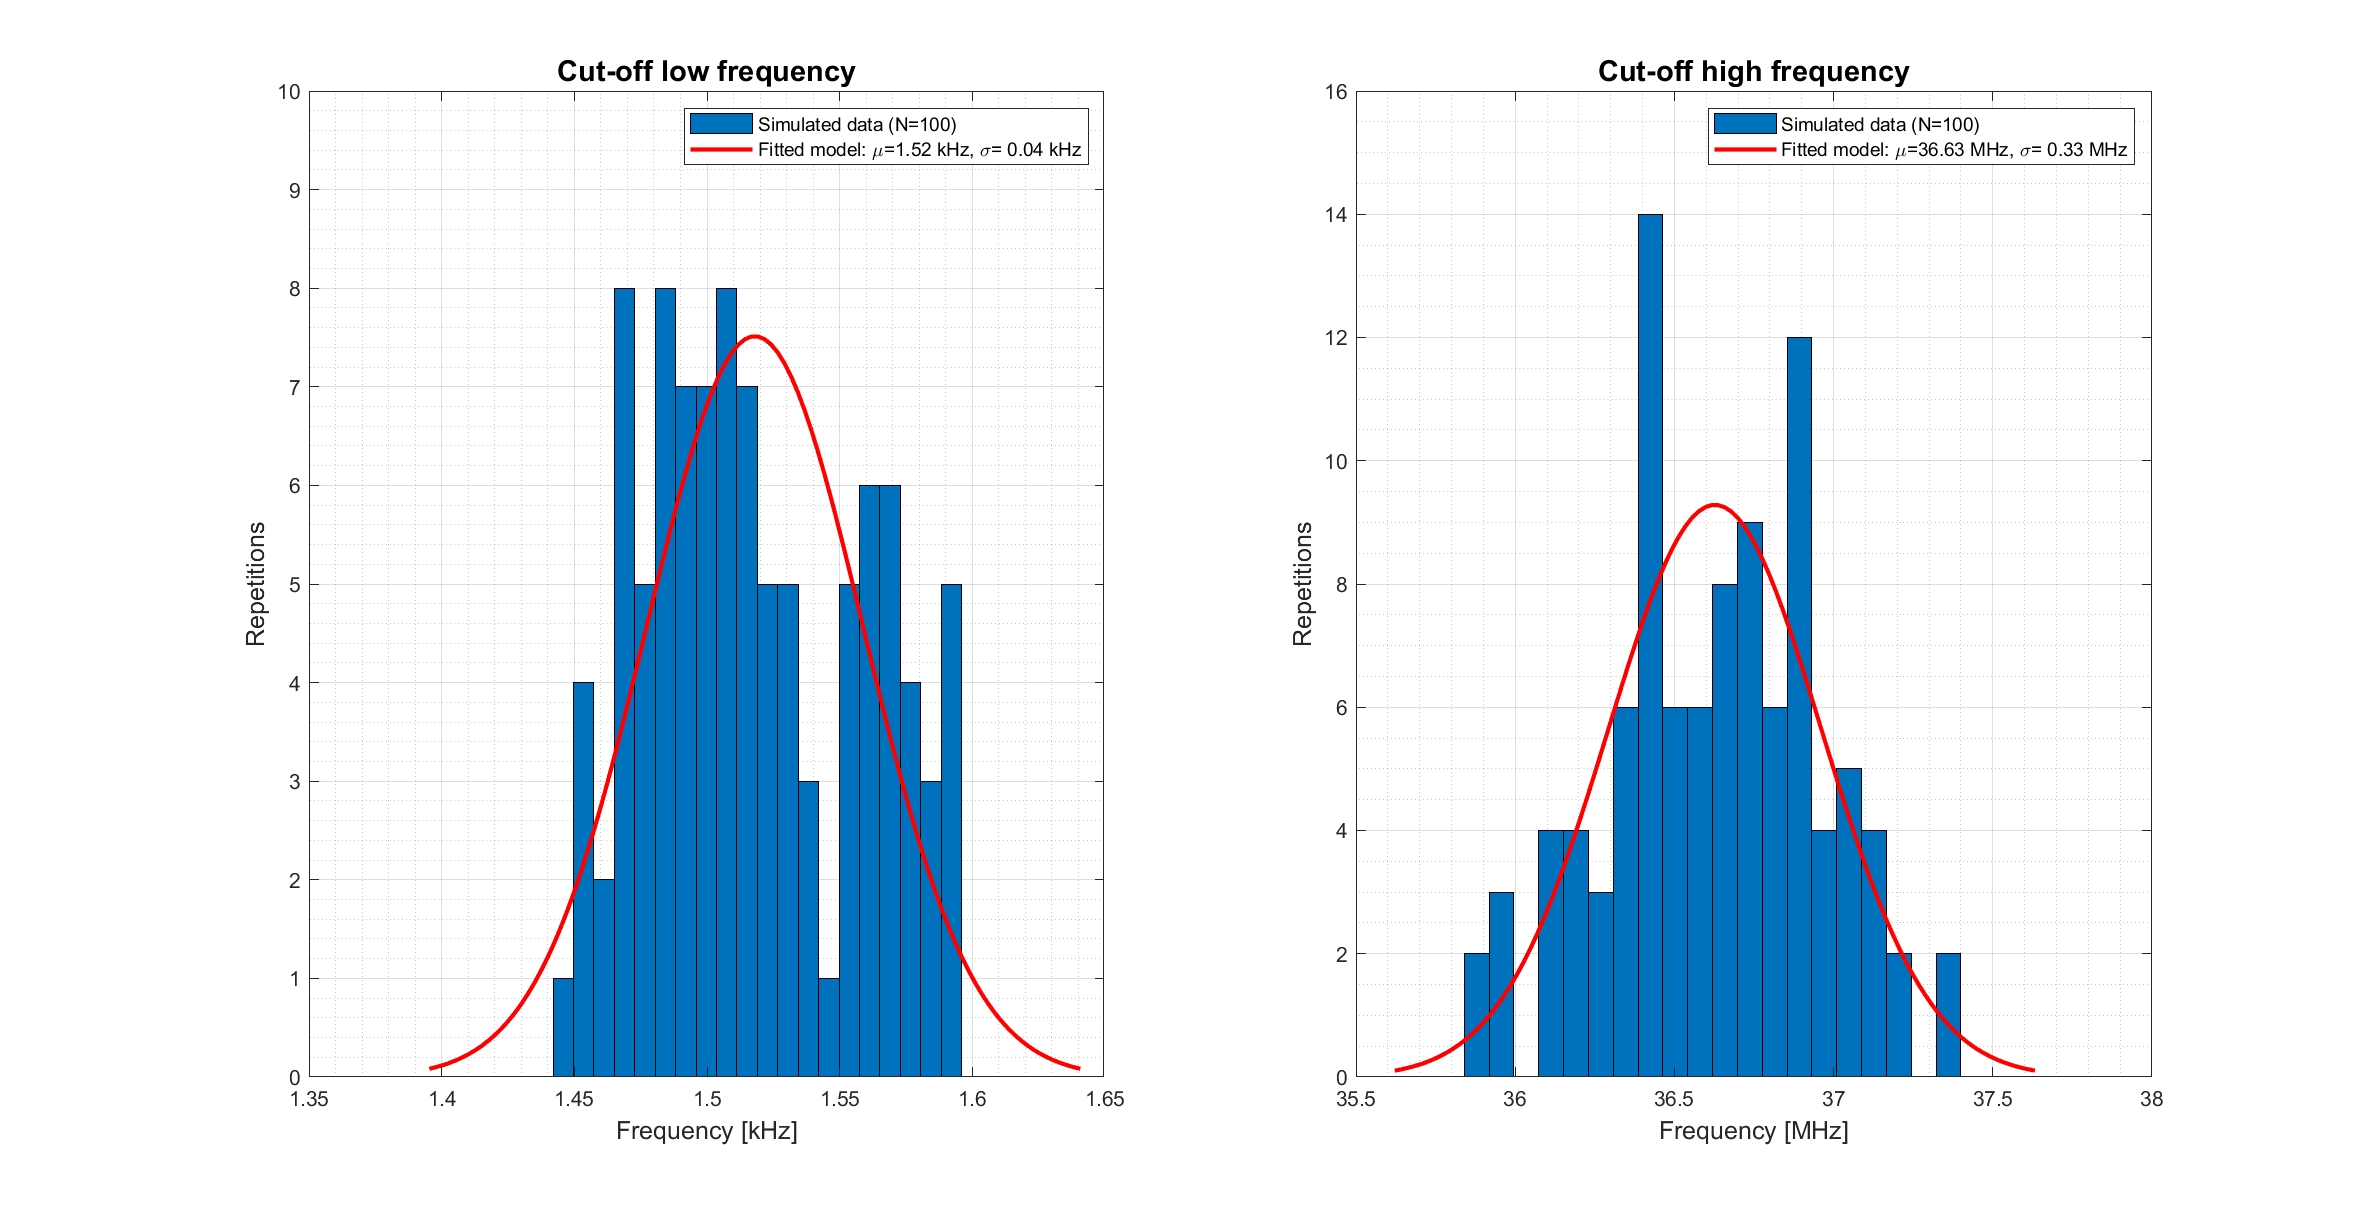
\includegraphics[width=\linewidth]{3_simulacion/fig/Hist_cir_act_100.png}
    \caption{Análisis estadístico de los lugares de los polos de bajas y altas frecuencias con carga activa, circuito real}
\end{figure}

\begin{figure}
    \centering
    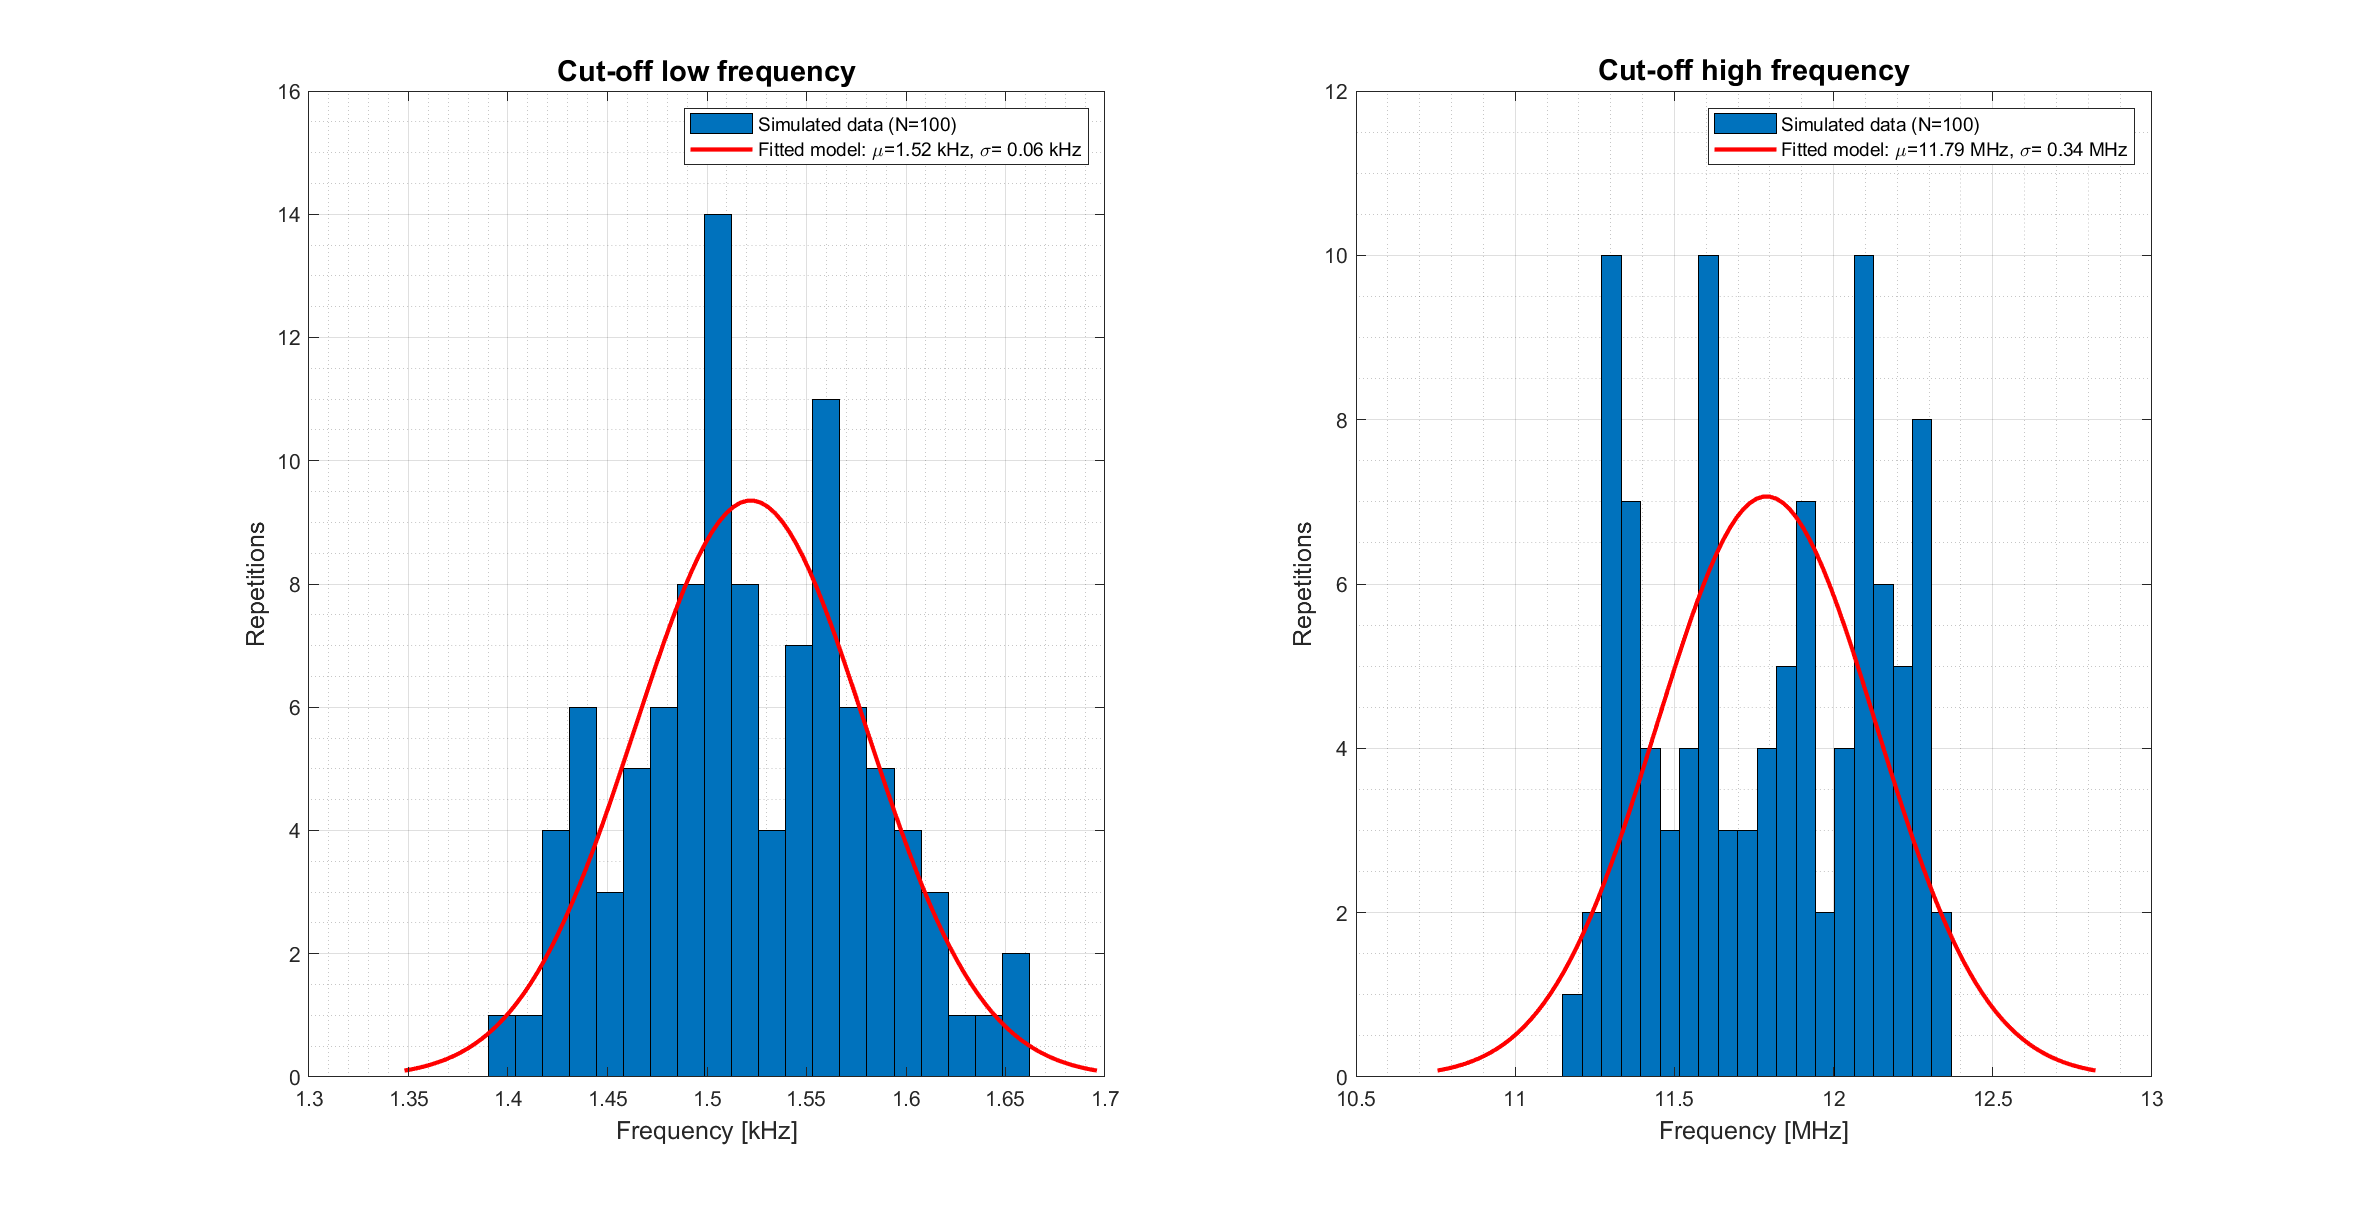
\includegraphics[width=\linewidth]{3_simulacion/fig/Hist_tb1_pas_100.png}
    \caption{Análisis estadístico de los lugares de los polos de bajas y altas frecuencias con carga pasiva, banco de pruebas 1}
\end{figure}

\begin{figure}
    \centering
    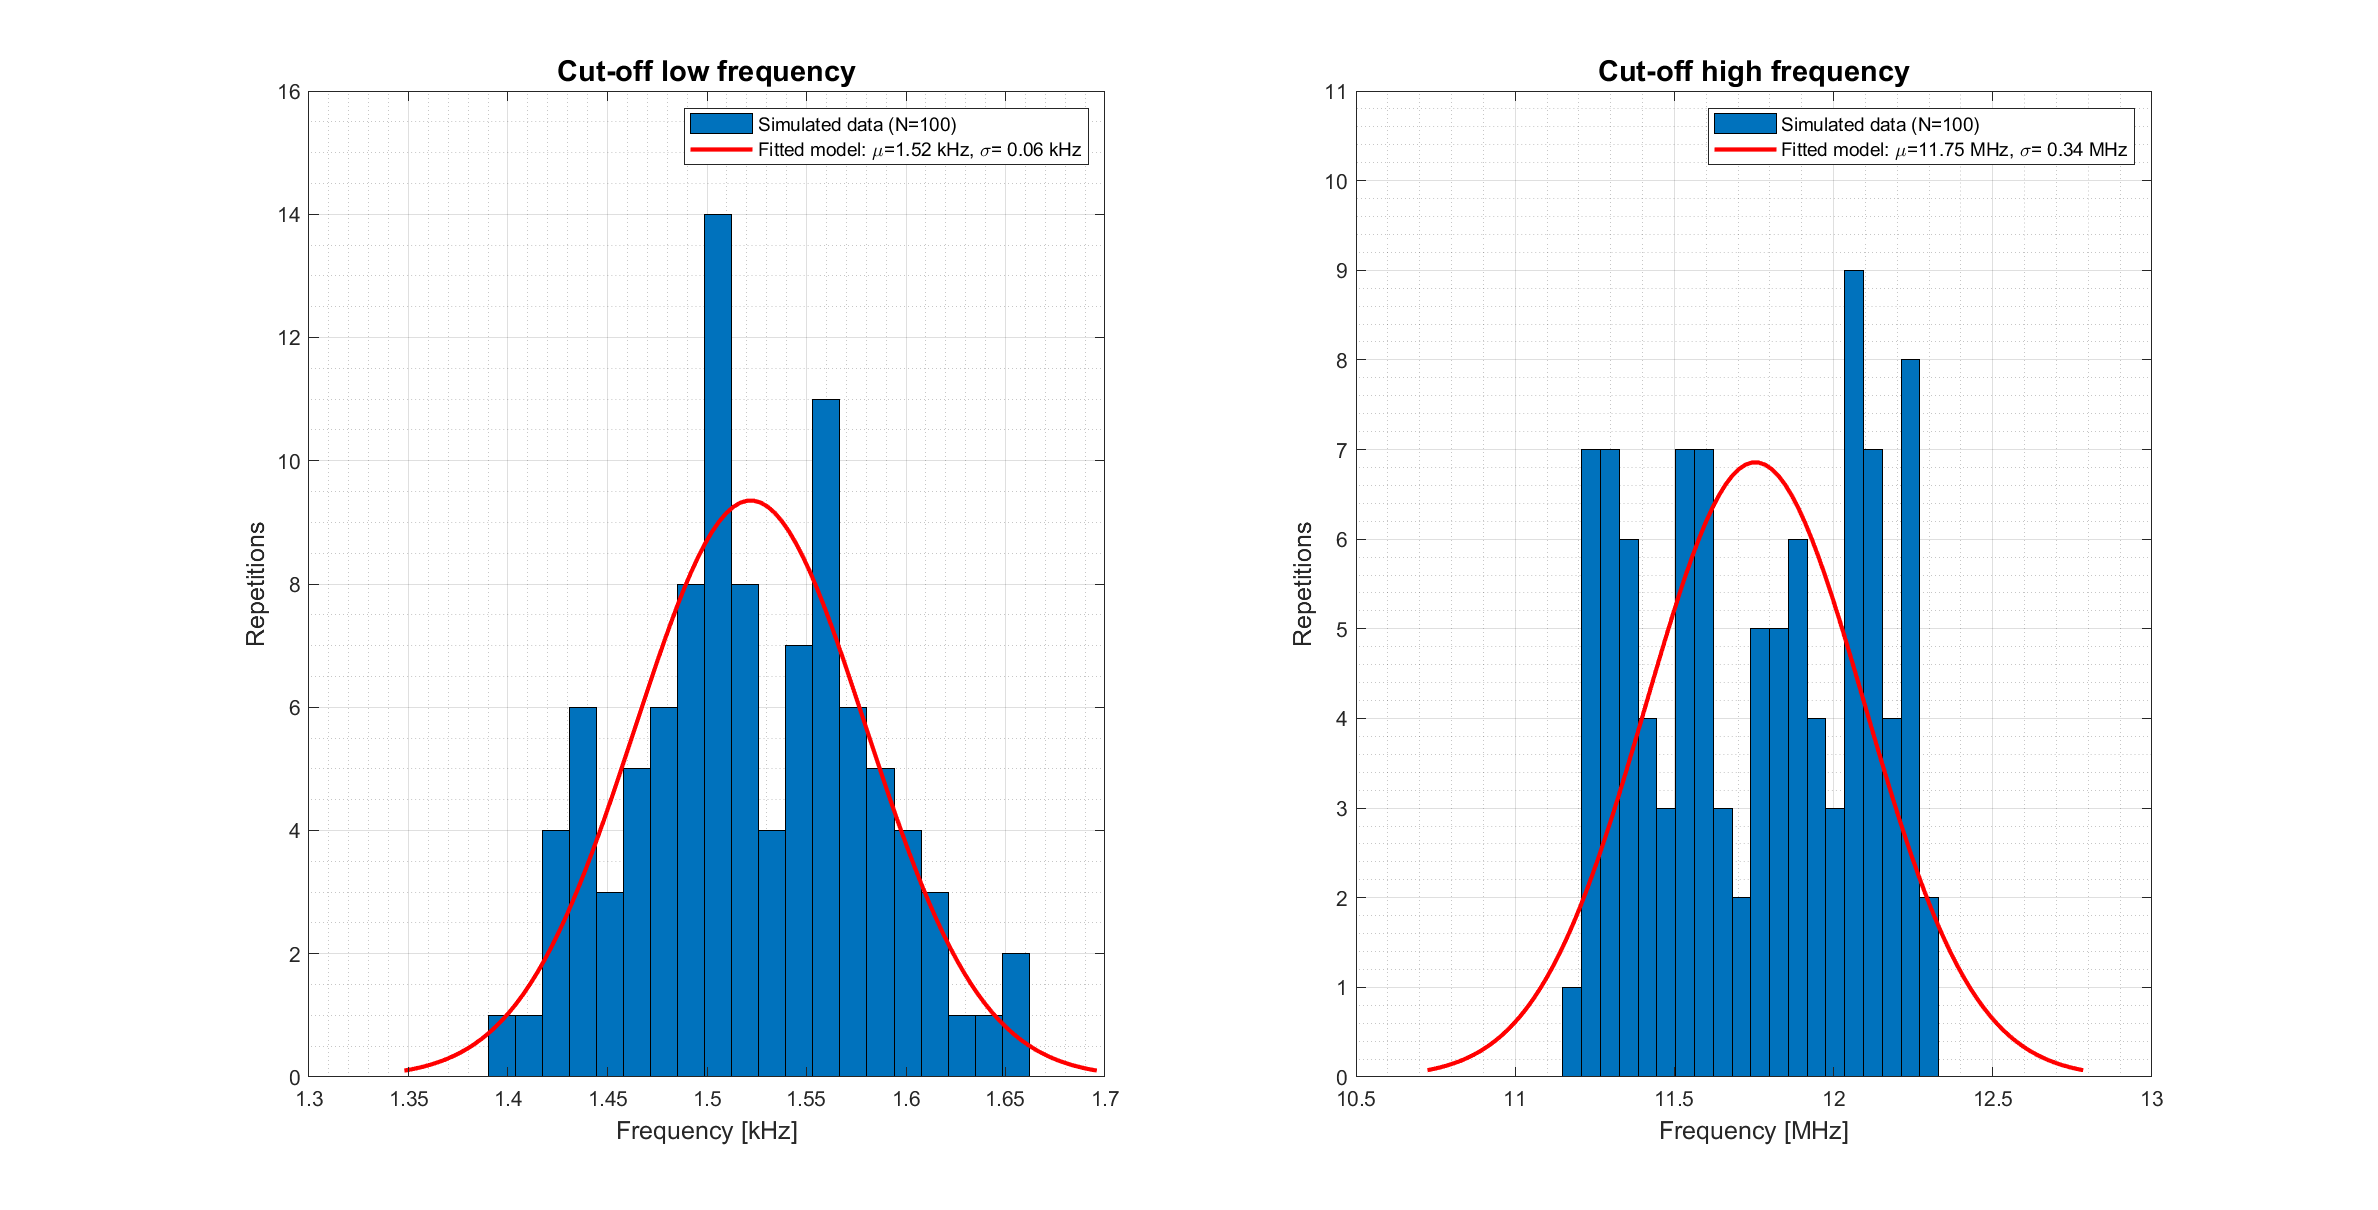
\includegraphics[width=\linewidth]{3_simulacion/fig/Hist_tb1_act_100.png}
    \caption{Análisis estadístico de los lugares de los polos de bajas y altas frecuencias con carga activa, banco de pruebas 1}
\end{figure}

\begin{figure}
    \centering
    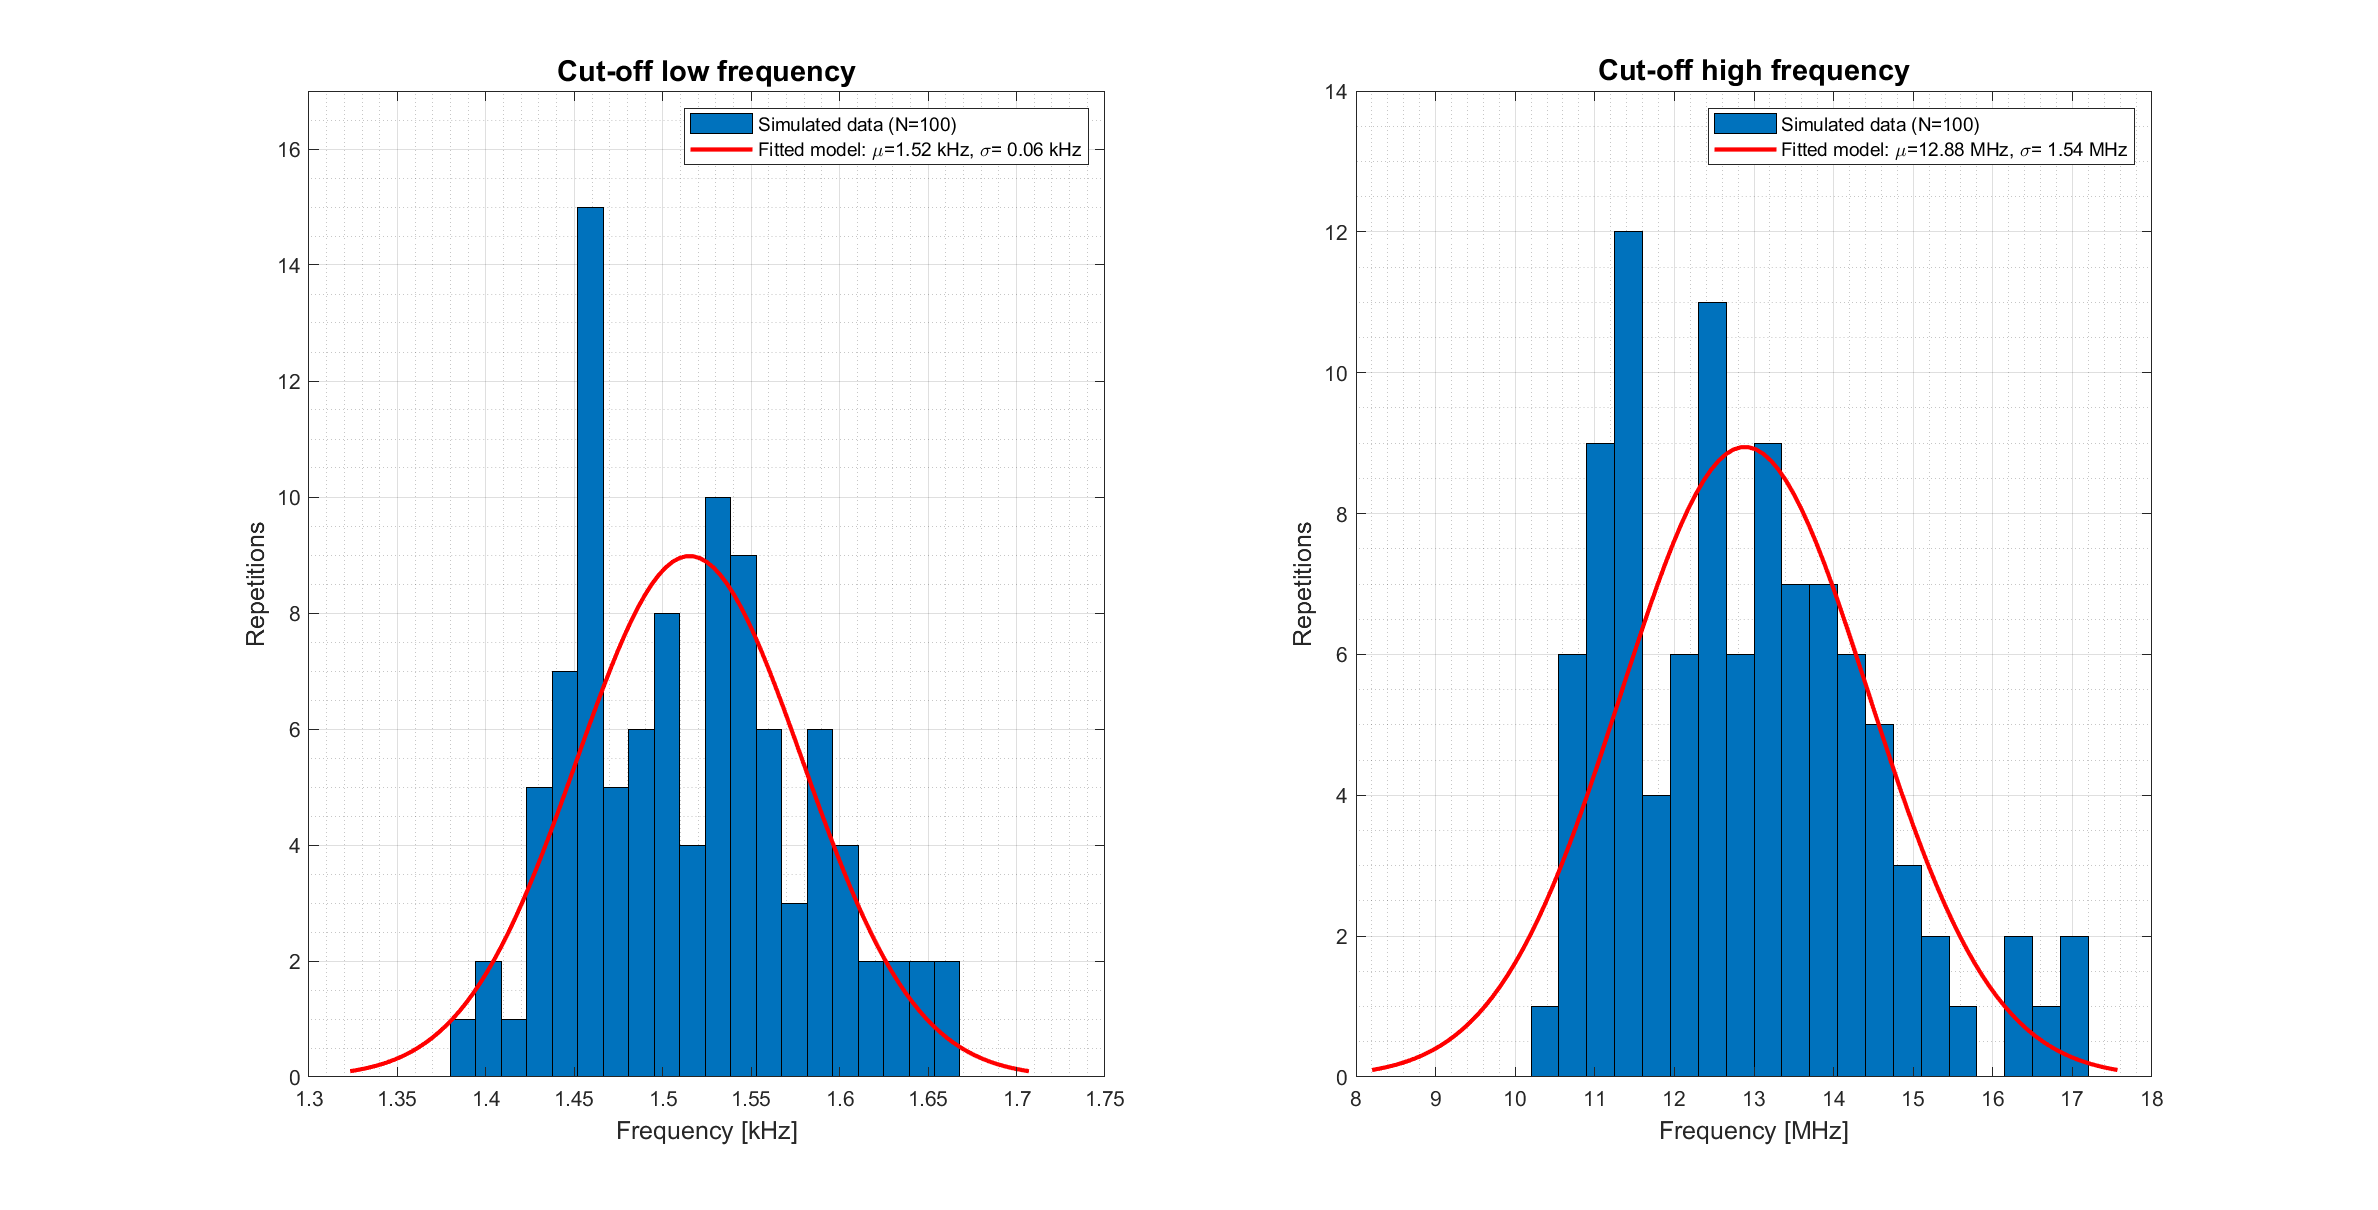
\includegraphics[width=\linewidth]{3_simulacion/fig/Hist_tb2_pas_100.png}
    \caption{Análisis estadístico de los lugares de los polos de bajas y altas frecuencias con carga pasiva, banco de pruebas 2}
\end{figure}

\begin{figure}
    \centering
    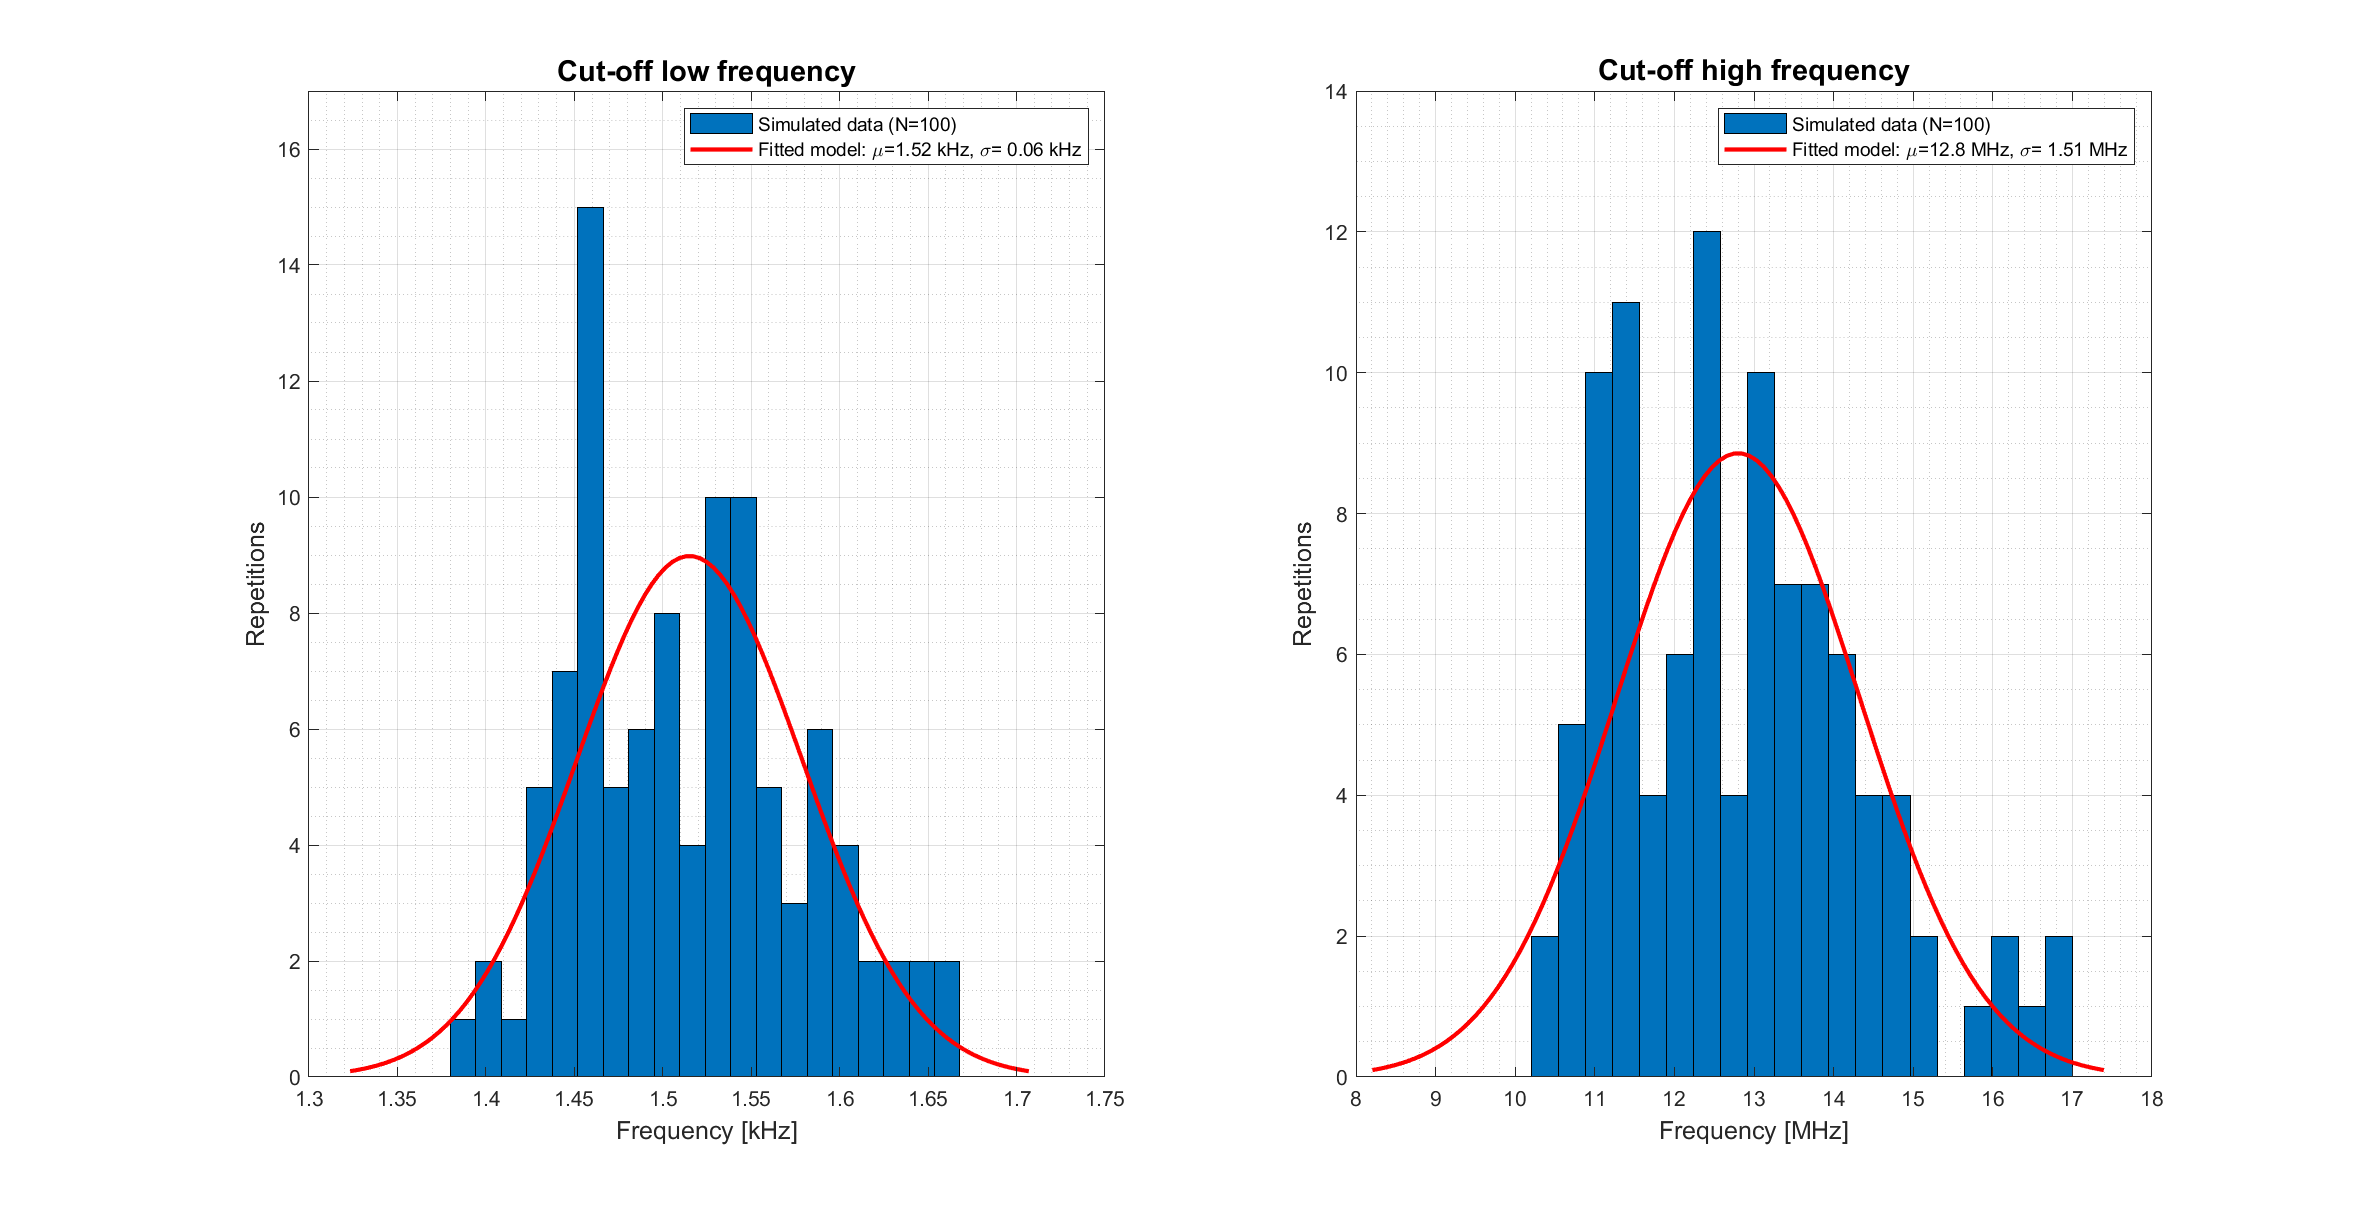
\includegraphics[width=\linewidth]{3_simulacion/fig/Hist_tb2_act_100.png}
    \caption{Análisis estadístico de los lugares de los polos de bajas y altas frecuencias con carga activa, banco de pruebas 2}
\end{figure}
